% AerE 3610 Lab Report Template
% Fall 2024
% Template by Professor Matthew Nelson

% Document Configuration DO NOT CHANGE
\documentclass{report}
% --------------------LaTeX Packages---------------------------------
% The following are packages that are used in this report.
% DO NOT CHANGE ANY OF THE FOLLOWING OR YOUR REPORT WILL NOT COMPILE
% -------------------------------------------------------------------

\usepackage{hyperref}
\usepackage{parskip}
\usepackage{titlesec}
\usepackage{titling}
\usepackage{graphicx}
\usepackage{graphviz}
\usepackage[T1]{fontenc} 
\usepackage{titlesec, blindtext, color} %for LessIsMore style
\usepackage{tcolorbox} %for references box
\usepackage[hmargin=1in,vmargin=1in]{geometry} % use 1 inch margins
\usepackage{float}
\usepackage{tikz}
\usepackage{svg} % Allows for SVG Vector graphics
\hypersetup{
	colorlinks=true,
	linkcolor=blue,
	urlcolor=cyan,
}
\usepackage{biblatex}
\addbibresource{myref.bib}
\usepackage{amsmath}
\usepackage{listings}
\usepackage{multicol}
\usepackage{array}

\usepackage{hologo} %KYR: for \BibTeX
\usepackage{algpseudocode}
\usepackage{algorithm}
% This configures items for code listings in the document
\usepackage{xcolor}

\definecolor{commentsColor}{rgb}{0.497495, 0.497587, 0.497464}
\definecolor{keywordsColor}{rgb}{0.000000, 0.000000, 0.635294}
\definecolor{stringColor}{rgb}{0.558215, 0.000000, 0.135316}
\definecolor{mygreen}{rgb}{0,0.6,0}
\definecolor{mygray}{rgb}{0.5,0.5,0.5}
\definecolor{mymauve}{rgb}{0.58,0,0.82}

\lstdefinestyle{customc}{
  belowcaptionskip=1\baselineskip,
  breaklines=true,
  frame=L,
  xleftmargin=\parindent,
  language=C,
  showstringspaces=false,
  basicstyle=\footnotesize\ttfamily,
  keywordstyle=\bfseries\color{green!40!black},
  commentstyle=\itshape\color{purple!40!black},
  identifierstyle=\color{blue},
  stringstyle=\color{orange},
 }
 
 \lstset{ %
  backgroundcolor=\color{white},   % choose the background color; you must add \usepackage{color} or \usepackage{xcolor}
  basicstyle=\footnotesize,        % the size of the fonts that are used for the code
  breakatwhitespace=false,         % sets if automatic breaks should only happen at whitespace
  breaklines=true,                 % sets automatic line breaking
  captionpos=b,                    % sets the caption-position to bottom
  commentstyle=\color{commentsColor}\textit,    % comment style
  deletekeywords={...},            % if you want to delete keywords from the given language
  escapeinside={\%*}{*)},          % if you want to add LaTeX within your code
  extendedchars=true,              % lets you use non-ASCII characters; for 8-bits encodings only, does not work with UTF-8
  frame=tb,	                   	   % adds a frame around the code
  keepspaces=true,                 % keeps spaces in text, useful for keeping indentation of code (possibly needs columns=flexible)
  keywordstyle=\color{keywordsColor}\bfseries,       % keyword style
  language=Python,                 % the language of the code (can be overridden per snippet)
  otherkeywords={*,...},           % if you want to add more keywords to the set
  numbers=left,                    % where to put the line numbers; possible values are (none, left, right)
  numbersep=8pt,                   % how far the line numbers are from the code
  numberstyle=\tiny\color{commentsColor}, % the style that is used for the line-numbers
  rulecolor=\color{black},         % if not set, the frame color may be changed on line breaks within the not-black text (e.g. comments (green here))
  showspaces=false,                % show spaces everywhere adding particular underscores; it overrides 'showstringspaces'
  showstringspaces=false,          % underline spaces within strings only
  showtabs=false,                  % show tabs within strings adding particular underscores
  stepnumber=1,                    % the step between two line numbers. If it's 1, each line will be numbered
  stringstyle=\color{stringColor}, % string literal style
  tabsize=2,	                   % sets default tab size to 2 spaces
  title=\lstname,                  % show the filename of files included with \lstinputlisting; also try caption instead of title
  columns=fixed                    % Using fixed column width (e.g. nice alignment)
}

\lstdefinestyle{customasm}{
  belowcaptionskip=1\baselineskip,
  frame=L,
  xleftmargin=\parindent,
  language=[x86masm]Assembler,
  basicstyle=\footnotesize\ttfamily,
  commentstyle=\itshape\color{purple!40!black},
}

\lstset{escapechar=@,style=customc}


\titlelabel{\thetitle.\quad}

% From here on out you can start editing your document
% ----------------------Page 1 Title Page------------------------------------------
% Make sure you edit your FirstName and LastName and the Lab number
\newcommand{\subtitle}[1]{%
  \posttitle{%
    \par\end{center}
    \begin{center}\LARGE#1\end{center}
    \vskip0.5em}%
}

\title{\textbf{Iowa State University
\\{\Large Aerospace Engineering 3610 \\Professor Nelson}}}
\subtitle{Report Example}
\author{Student: FirstName LastName}

\begin{document}
\maketitle
\tableofcontents
% ----------------------Page 2 Intro, Objectives and Methodology-----------------------------------
\chapter{About this Example}
This document is an example and is meant to be your template for all future reports. Except for this chapter (the ``About this Example'' chapter), you must keep all chapters and sections as they are in this document. We have briefly described what we expect in each chapter and section. We have also provided several examples of how to add certain things like images, tables, equations, and even your code into your lab reports. Any other specific requirements will be outlined in the mission write-up. 


\section{Introduction}
Your introduction is your need and problem stated in general terms. This should be an overview of your report and be brief. This section should be 1-2 paragraphs long.

\begin{tcolorbox}
\emph{Hints:} \\
Your professor considers a ``paragraph'' to be at least three complete sentences. Most paragraphs should not exceed ten sentences. Also, this is an example of adding a tcolorbox if you need to use one.
\end{tcolorbox}

\section{Objectives}
Outline the objectives that you worked on. Look at the mission write-up and the homework for this information, but do not simply copy and paste from there. This section should be 1-2 paragraphs long.

\section{Methodology}
This is your approach to how you attempted to solve the problem stated for the homework. You should include what tools you used (IDE, compilers, etc.) and why. You should also state any other sources you used (mission write-up, lectures, book materials, websites, etc.). This section will be pretty short (and probably fairly repetitive) for the first few homework. But as we use new tools and get into more complicated homework, this will be expanded. To start, I would expect about a paragraph. Later, this might be two paragraphs.

% ----------------------Page 3 Results-------------------------------------------
\chapter{Work Summary}

\section{Results}
This section displays what your program(s) did, including any outputs or information generated by the program. The mission write-up may also state if this section should contain certain information. Below are examples of how you should format certain items for this report, such as code outputs, tables, images, and code snippets.

%-----------------------------Code output example--------------------------------------
\subsection{Code Outputs}
Often, you will be asked to show the output your code displays on the screen. Do not take a screenshot of your screen! Instead, you can save the output to a text file or copy it to your report. To format this, we will use a box. Please copy and paste your output for this lab to replace what we have.

\begin{tcolorbox}
\emph{Code Output:} \\
INSERT YOUR OUTPUT HERE
\end{tcolorbox}

\subsection{Lists}
There are two types of lists, enumerated (numbers or letters) and bulleted lists. Below are some examples of those lists.

\textbf{Bulleted Lists}
\begin{itemize}
    \item Item number 1
    \item Item number 2
    \item Item number 3
\end{itemize}

\textbf{Numbered}
\begin{enumerate}
    \item Item number 1
    \item Item number 2
    \item Item number 3
\end{enumerate}
 %-------------------------------------------Tables Example (Start)-----------------------------------------------
\subsection{Tables}
You may be asked to generate some tables to show data generated by your program. For that, we use \texttt{tabular} to generate them. Some examples are given below. It would be best if you always referenced your tables in your writing. To do that, you would reference it like this: Table \ref{table:command}. Note that what you place in the \verb!\label! is how you call this; you need a unique name for each label. We do this by putting what the label is first and then using a colon. Note that for this label, we have \texttt{table:command}, and for Table \ref{table:gauss} we have a new name.
%%Example-1
\begin{table}[ht]
\label{table:command}
\caption{Command option table.}
\begin{tabular}{|c|c|p{4.2in}|}

\hline
Command & Option & What this command/option combination does \\
\hline
\hline
\texttt{gcc} & -o & To \emph{generate} an executable for the source c code.\\
\hline
\texttt{./<name>} & N/A & To \emph{instruct} it to run the program called name in the \emph{current directory}\\
\hline
\end{tabular}
\end{table}

%%Example-2

\begin{table}
\caption{Brute force table.}
\label{table:gauss}
\begin{center} \begin{tabular}{|c|r|r|}
\hline
$n$ & Brute Force Time & Gauss Adder Time \\
\hline
\hline
1 & 1s & 2s\\ \hline
10 & 10s & 20s\\ \hline
100 & 20s & 30s\\ \hline
\end{tabular} \end{center}
\end{table}

%-------------------------------------------Tables (End)-------------------------------------------------
\subsection{Images}

\ref{eq:1}
Some missions may output information as an image; you will want to include those in your reports. Images are treated a little bit differently in \LaTeX. For images, we place them in a figure and then include the image. It would be best if you also referenced your figures as well. You do that like this: Figure \ref{fig:361_demo}. \LaTeX will automatically insert the correct number (this is a huge benefit to using \LaTeX!). Like with tables, make sure your labels are unique, and typically, we use \texttt{fig:} to label our labels.

All images must be placed in the \emph{images} folder. Right now, there is one image there that we placed there for you. To add a new image, we need to upload it to Overleaf. This is easy to do. Click on the \emph{images} folder and then click on the three dots to the right of the folder name. There, you will see an option to upload a file.

\begin{tcolorbox}
\emph{Hint:} \\
An upload button is also located just above the directory listing in Overleaf. While you can use this, it will place files in the root folder. That is not a big deal; you can move the file into the images folder after it is uploaded. Using an images folder is also not required as we have done. But it does help to keep your directory organized.
\end{tcolorbox}
%--------------------------------Image example--------------------------------------

\begin{figure}[ht]
\centering
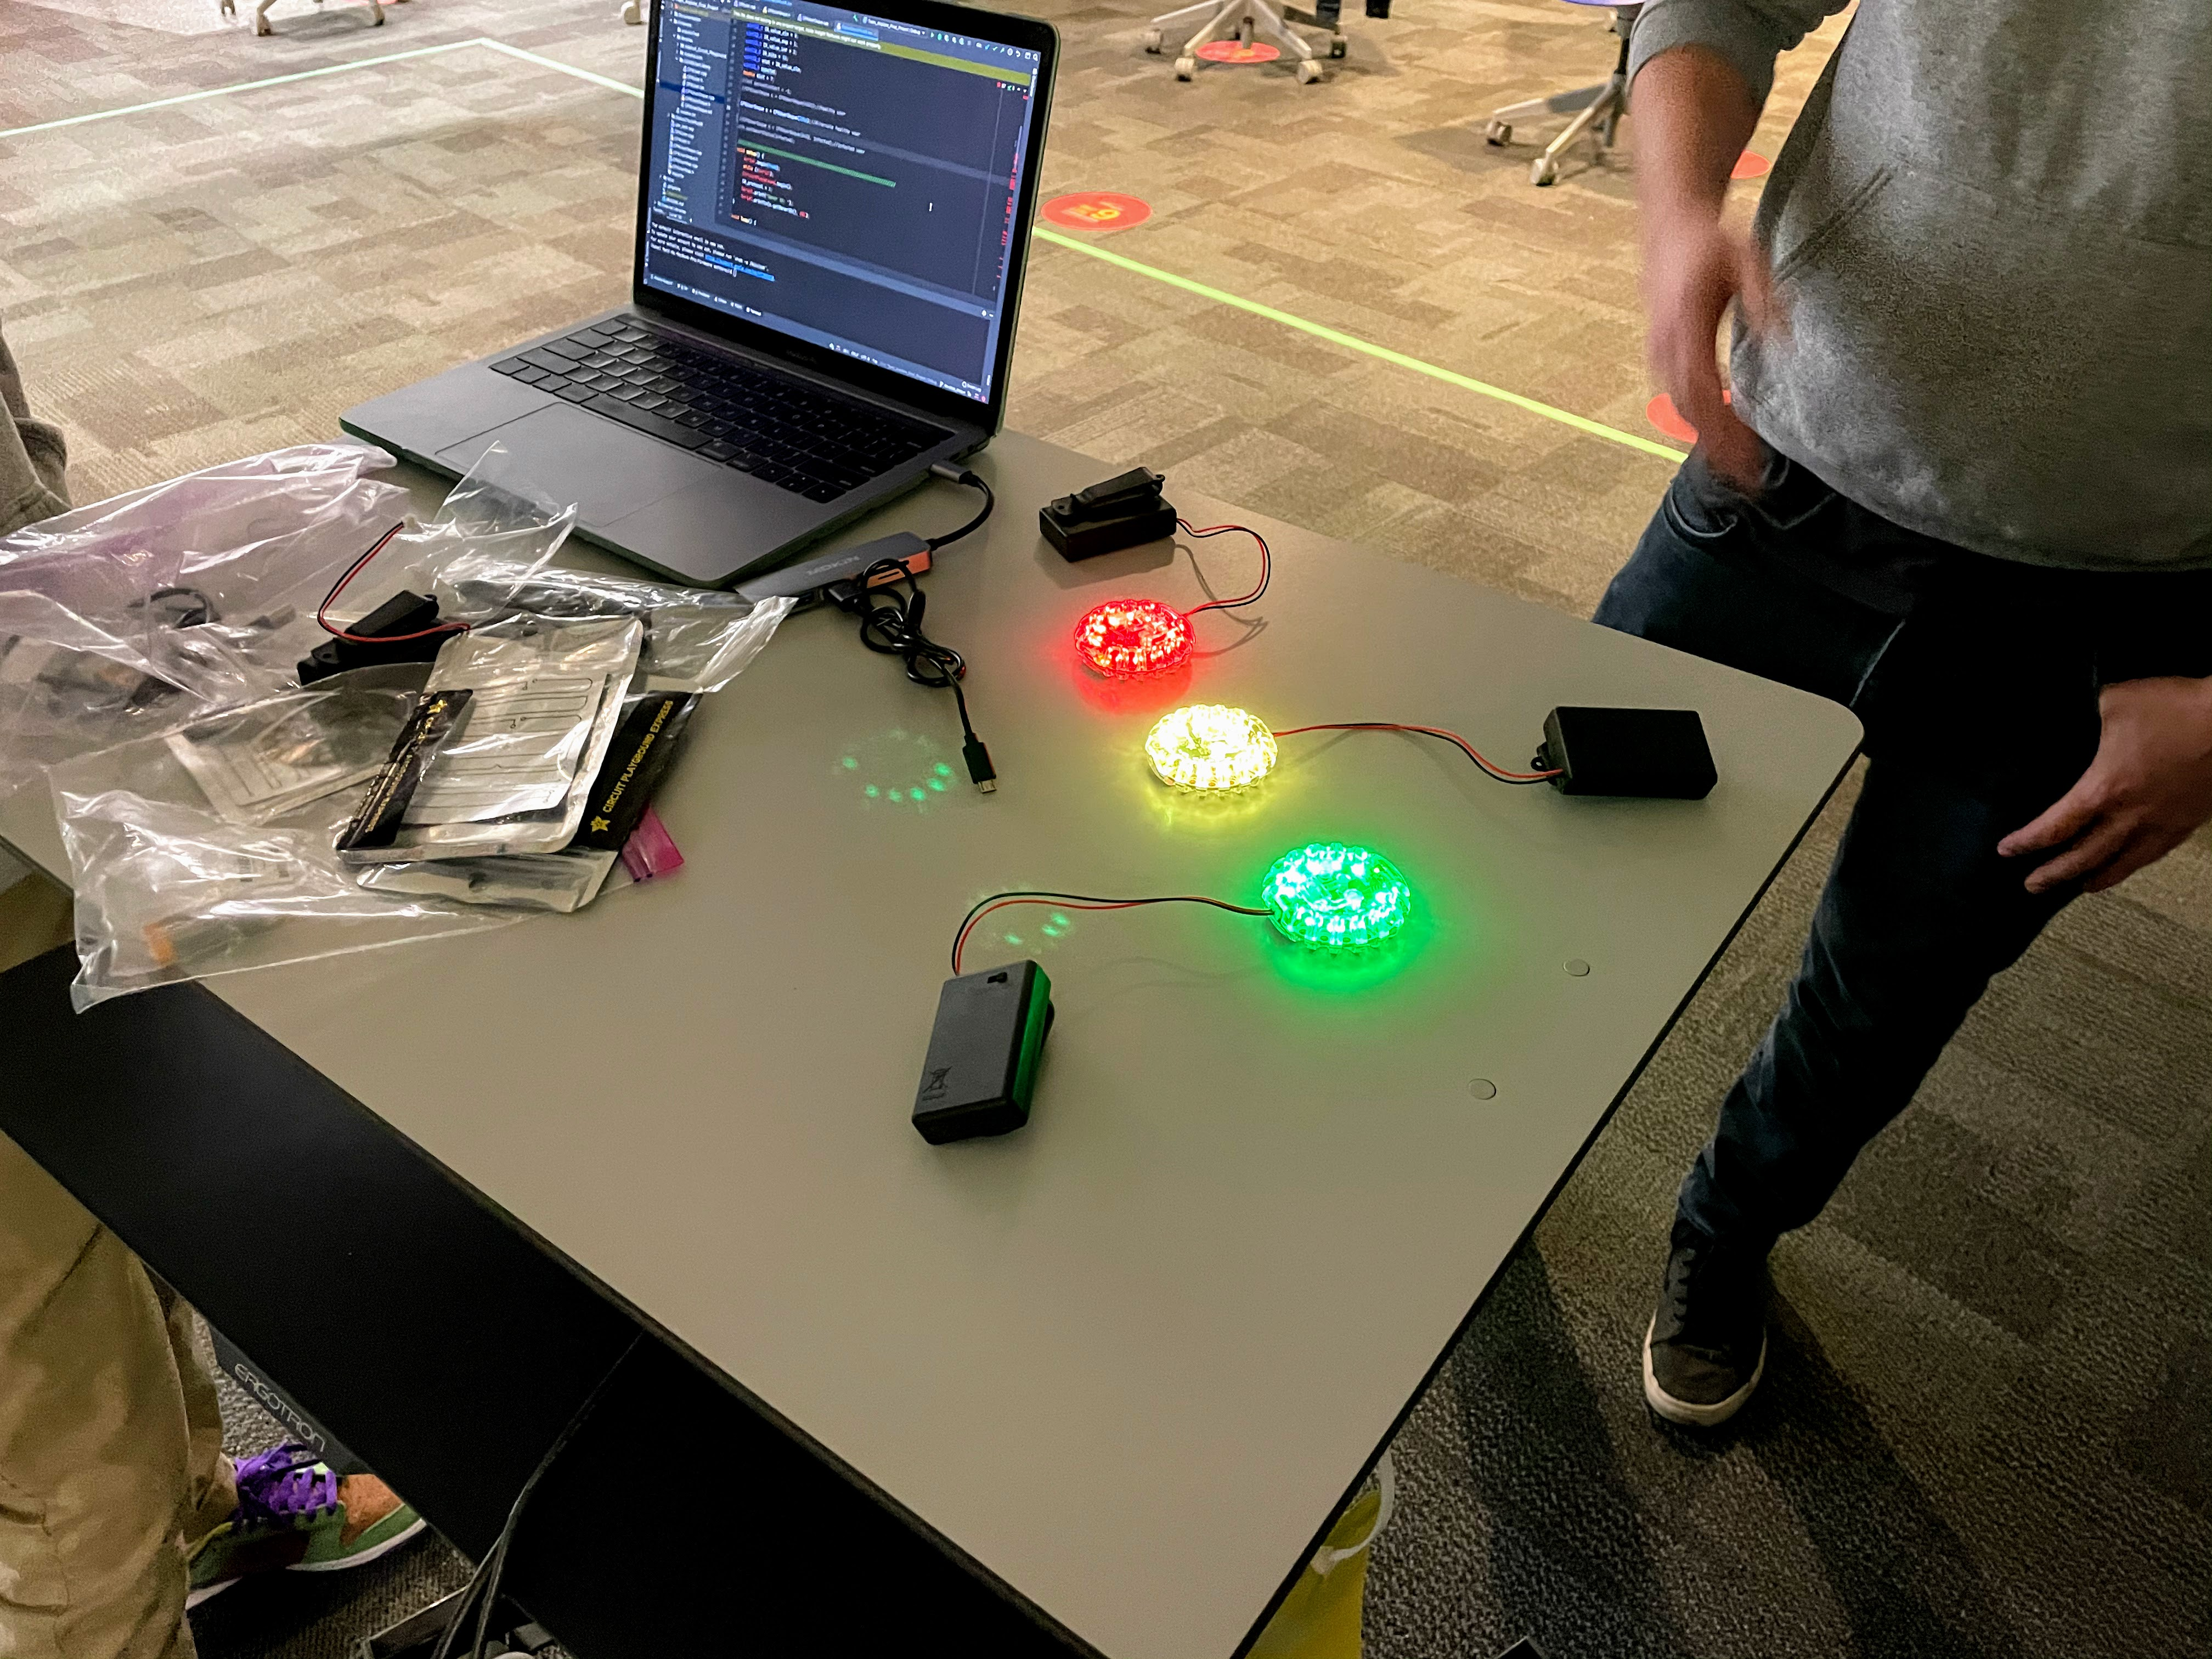
\includegraphics[width=6in]{images/IMG_0038.jpg}
\caption{Students in the Fall 2020 AerE 361 demoing their projects.}
\label{fig:361_demo}
\end{figure}
%-------------------------------End Image example

%-------------------------------Inserting source code
\subsection{Code}
All source code must go in the \texttt{src} directory. Once there, you can call your source code as shown in Listing \ref{code:ex1}. In that example, we can specify a range of line numbers to display. If we remove those, the entire code will be displayed.
\ \\
\lstinputlisting[label={code:ex1}, caption={Example of listing only certain lines of code from a file.},language=Python, firstline=1, lastline=19]{src/example.py}

You can also list your code as shown in Listing \ref{code:ex2}.
\begin{lstlisting}[language=C,caption={Example of listing code directly},label=code:ex2]
#if defined(FIT_CONVERT_MULTI_THREAD)
    		FitConvert_Init(&state, FIT_TRUE);
	#else
    		FitConvert_Init(FIT_TRUE);
	#endif

\end{lstlisting}
If you use a different programming language, you can also change that. This is shown in Listing \ref{code:ex3}. Note that in Overleaf, the \verb!\ref{}! the command will not automatically see the labels, and therefore, it will not do an auto-complete like with tables and figures.

\begin{lstlisting}[language=Python,caption={Python example},label=code:ex3]
a = 33
b = 33
if b > a:
  print("b is greater than a")
elif a == b:
  print("a and b are equal")

\end{lstlisting}


\section{Analysis}
The analysis is your interpretation of the information generated. This requires you to think about the results and give us your thoughts. The mission write-up will also ask several questions, and your responses to those, in many cases, will be placed here. You may also need to cite where you are getting some of this information. For that, we have provided an example bibliography file that you can use. For example, this report is based on the book \emph{Writing Style and Standards in Undergraduate Reports} by Jeter, Sheldon Moseley et al. \cite{jeter2016writing}. You will notice that the citation for this is in the Reference section at the end of our document. You will not need to cite in every report, but the final project will require some citations. 

Below are some examples of how you might be asked to answer some questions or how to list out your analysis for your mission report. Note in Exercise 1, we are using an equation. Like everything else, this needs to be referenced as well. That is easily done like this: Equation \ref{eq:1} or like Equation \ref{eq:2}. Equations do not have captions with them and are instead automatically numbered in order.
\subsection{Exercise-1}
%Insert equation
\begin{equation}
\label{eq:1}
123 + 567 = 690
\end{equation}

\begin{equation}
\label{eq:2}
    \int_{\partial \Omega} \omega = \int_{\Omega} d \omega
\end{equation}

For this problem, \texttt{unsigned int} for b = 567 should change to \texttt{unsigned short} because it would be a better fit for the value range. For the second line, \texttt{unsigned char} needs to change to \texttt{unsigned short} since the range is greater than 255.

\subsection{Exercise-2}
It will be $O{_{\mathrm(n)}}$, because the size is n, so the loop iterates n times in the worst-case scenario could take less time.

\chapter{Conclusion}
\section{Summary}
Your summary should wrap up your report and re-state any key conclusions you came up with. A good summary should be well thought out but concise. I would expect around 2-3 paragraphs.
\section{Reflection}
Each module will ask reflection questions, and you will answer those questions here. For this report, answer the following questions.

\begin{enumerate}
    \item This mission and report focused on writing and doing a report you will do for future modules in this class. Reflect on what tools you have used to write reports and how those differ (or maybe the same) from the reports we will do in this class.
    \item What are some things you learned from doing this mission? List out what you learned and how you hope to use them.
\end{enumerate}
\section{References}
Your references will automatically be generated below (this sentence should be deleted).
\printbibliography[heading=subbibintoc]

\end{document}